\begin{frame}{Examples: Comparison between methods}

    \begin{itemize}
        \item MSA of distantly related globins (human beta globin, human myoglobin, human neuroglobin, soybean leghemoglobin, rice hemoglobin) using four different programs. Symbols: * complete conservation, : conservative substitutions, . less conservative substitutions. Programs differ in:
        \begin{itemize}
            \item Align corresponding regions of alpha helical secondary structure (red lettering).
            \item Align conserved histidines (open and black arrowhead). They are important in coordinating protein binding to the heme group $\rightarrow$ they should be aligned by all the programs. The open arrowhead histidine shows a complete conservation. The conservation of the black is only achieved by ProbCons and T-Coffee.
            \item Create and place gaps (boxed regions).
        \end{itemize}
    \end{itemize}
            
\end{frame}

\begin{frame}

    \begin{figure}[t]
        \raggedleft
        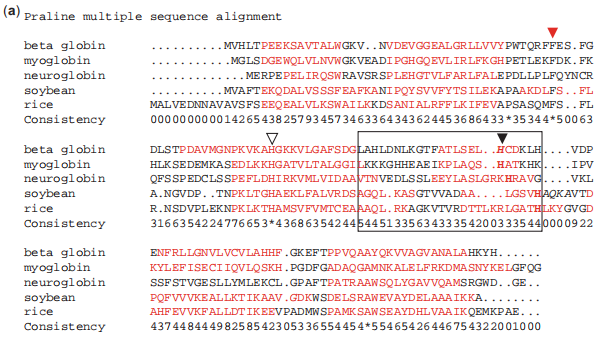
\includegraphics[width=0.49\textwidth]{./img/Comparacion_1.png}
        \raggedright
        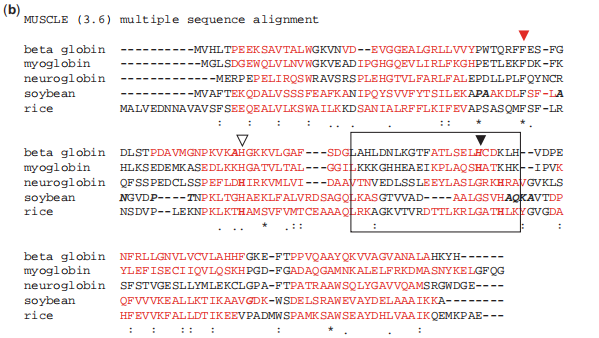
\includegraphics[width=0.49\textwidth]{./img/Comparacion_2.png}
    \end{figure}
    \begin{figure}[b]
        \raggedleft
        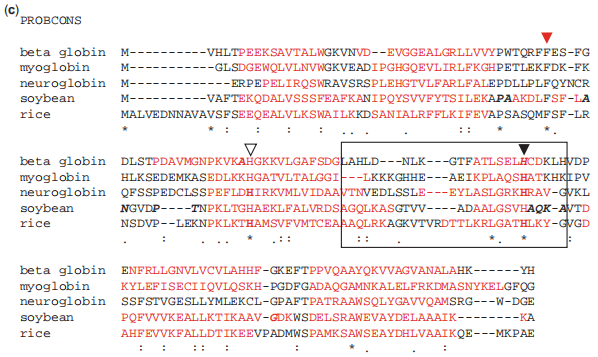
\includegraphics[width=0.49\textwidth]{./img/Comparacion_3.png}
        \raggedright
        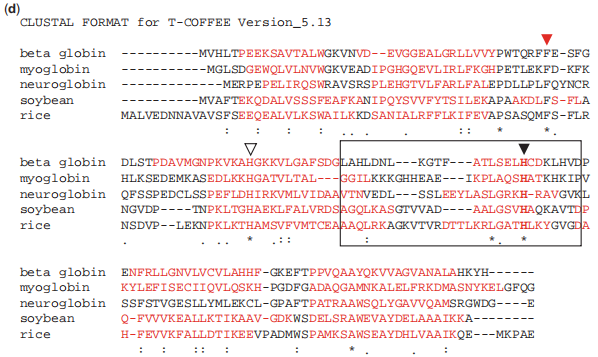
\includegraphics[width=0.49\textwidth]{./img/Comparacion_4.png}
    \end{figure}

\end{frame}